%% LyX 1.1 created this file.  For more info, see http://www.lyx.org/.
%% Do not edit unless you really know what you are doing.
\documentclass[prb,aps,twocolumn]{revtex4}

\usepackage{graphicx}
\usepackage{amsfonts}
\usepackage{amsmath}
\usepackage{bm}
\usepackage{alltt}
\usepackage{dcolumn} 
\usepackage{amsmath} 
\usepackage{graphicx}
\makeatletter 
\makeatother

\begin{document}

\title{\textbf{Linear scaling computation of the Exchange-Correlation matrix. Gaussian
orbital methods for simulation of periodic systems}}


\author{C. J. Tymczak}
\author{Matt Challacombe}

\affiliation{Theoretical Division, Los Alamos National Laboratory, Los Alamos,
New Mexico 87545 }

\date{\today}

\begin{abstract}
Periodic boundary conditions have been implemented in the linear scaling
Quantum Chemistry code \textbf{MondoSCF}. For the two-electron Coulomb
matrix, this has been achieved with an exact multi-pole expansion of
the long range Coulomb field. This yields a spherically summed boundary
condition that is easily transformed to Ewald boundary conditions.
In order to achieve linear scaling of the local Coulomb field, a Quantum
Chemical Tree Code (QCTC) is used. Periodic boundary conditions have
also been incorporated into calculations of the local exchange-correlation
matrix and the exact-exchange matrix. A Hierarchical Cubature (HiCu),
pure Cartesian adaptive grid is used for the local exchange-correlation
matrix. This method achieves linear scaling through the use of advanced
data structures (k-d trees) that maximally exploits locality of the
density. Finally, the current capabilities of \textbf{MondoSCF} for large condensed
phases will be demonstrated.
\end{abstract}

\maketitle

\section{INTRODUCTION}
In recent years several successful methods for the calculating the electronic structure of
molecular or condensed matter systems have been developed,
for example Hatree-Fock \cite{Slater51,Roothaan51}, Density Functional theory 
\cite{Hohenberg64,KohnSham65} or Configuration interaction \cite{Choudhury79}. 
All these methods attempt to solve for the electronic structure via
the many-body quantum problem to within some consistent approximation scheme.
For complex molecular or condensed matter 
system, where chemical reactions are of central importance, these electronic structure
method are essential. Unfortunately, most electronic structure quantum chemistry codes
scale very poorly with system size due to the need to diagonalize the Hamiltonian,
which scales $O(N^3)$ 
\cite{???}.
%
% Should cite standard comercial code like ``Gaussian''. (Ha)
%
This severely limits the systems sizes 
that these codes can address. Therefore, it has become increasing important for
the development of quantum chemistry codes which scale linearly with increasing 
system size, and several quantum chemistry codes of this type are in 
development 
\cite{Goedecker94,Challacombe96,Canning96,Briggs96,Hernandex96,Scuseria99,ANiklasson02}. 
However, for reasons of simplicity most of these quantum 
chemistry codes have yet to incorporate periodic boundary conditions.
Unfortunately many
technically important systems can only be addressed within a condensed phase environment,
where surface effects have been removed \cite{Allen90}. Therefore, the inclusion of 
periodic boundary conditions into existing linear scaling quantum chemistry
codes is essential. 

We have implemented periodic boundary conditions into the linear scaling
quantum chemistry code \textbf{MondoSCF} 
\cite{Challacombe96,Challacombe97,Challacombe99}.
For the one electron matrix this has been achieved by a re-summation
over periodic cell images, which because of locality leads to an efficient
calculation of the one electron matrices. For the two electron matrices
various methods are employed. For the two-electron Coulomb matrix,
we achieve this via an exact multi-pole expansion of the long range
Coulomb field \cite{White94,Challacombe97b}. This yields a spherically
summed boundary condition that is easily transformed into the Ewald boundary
condition \cite{Redlack72,Redlack75}. In order to achieve linear
scaling of the local Coulomb field, a Quantum Chemical Tree Code (QCTC)
is used \cite{Warren93,Warren95,Salmon94,Challacombe96A}. For the calculations of the 
local exchange-correlation matrix, a Hierarchical Cubature (HiCu), pure 
Cartesian adaptive grid
is used. This method achieves linear scaling through the use of advanced
data structures (k-d trees) that maximally exploits locality of the
density, and allows for an efficient treatment of the periodic effects
\cite{Bentley79}. All \textbf{MondoSCF} calculations are done at the gamma-point.
This is because the main focus of the \textbf{MondoSCF} linear scaling quantum chemistry
code is large systems, where for insulators k-space integrations become unnecessary 
\cite{Nunes94}.


To demonstrate and validate the capabilities of \textbf{MondoSCF}, we show results for 
three condensed phase systems, Sodium Chloride, Magnesium Oxide 
and Carbon in the diamond structure. We then compare these results to the periodic
Gaussian code \textbf{Crystal98} \cite{Crystal98}. Next we demonstrate that
the code achieves {\it true} linear scaling for the dense periodic diamond system 
up to 512 atoms in the unit cell.
%
% Example system
%
To show the full capabilities of \textbf{MondoSCF} we calculate the surface reconstruction
of the Silicon (111) surface with a step.
%
Finally we give some conclusion concerning the accuracy and utility of \textbf{MondoSCF}
and future research directions.

\section{The Kohn-Sham Equations}

Following the seminary work of Kohn and Sham\cite{KohnSham65}, we start with the KS single 
particle equation
\begin{equation}
H \phi_{i}({\bf r})  = \epsilon_i \phi_{i}({\bf r})
\end{equation}
where the effective Hamiltonian is
\begin{equation}
H = -{\nabla}^{2}+ V_{ext}({\bf r}) + J[\rho({\bf r})] + K_{xc}[\rho({\bf r})]
\end{equation}
and
\begin{equation}
 \rho({\bf r}) = \sum_{i=1}^{N_{el}} | \phi_{i}({\bf r}) |^2
\end{equation}
\begin{equation}
 J[\rho({\bf r})] = \int d{\bf r'} {\rho({\bf r}) \over |{\bf r}-{\bf r'}|},
\end{equation}
and the exchange correlation potential can be calculated from several approximate
functionals
\cite{Becke92,Hertwig97,Bauschlicher95,Adamo00}. In what follows we will 
discuss the calculation of each of the terms in the Hamiltonian 
and how they are calculated in the non-orthogonal Gaussian basis
with the inclusion of periodic boundary conditions.

\section{One-Electron Matrices}

The first step in including periodic boundary conditions into our
linear scaling code is to determine the minimal modifications to the
one-electron integrals needed to obtain this. We incorporate periodic
boundary conditions into our linear scaling method by modifying the
integrals. Consider the non-periodic overlap matrix

\begin{equation}
\label{Sab_norm}
S_{ab}=\int _{V_{\infty }}\, d{\mathbf{r}}\, \phi _{a}({\mathbf{r}})\phi _{b}
({\mathbf{r}})
\end{equation}
 where \( \{\phi _{a}(x),\phi _{b}(x)\} \) are the atomic orbitals
(LCAO) at atom \( a \) and atom \( b \) and \( V_{\infty } \) is
the integration over all space. In the periodic case this is replaced
by,

\begin{equation}
\label{Sab_pbc1}
S_{ab}^{PBC}=\sum _{\mathbf{R},\mathbf{R}'}\int _{V_{cell}}\, d{\mathbf{r}}\, 
\phi _{a}({\mathbf{r}+\mathbf{R}})\phi _{b}({\mathbf{r}+\mathbf{R}'})
\end{equation}
where, \( V_{cell} \) is the integration over the simulation cell,
and \( \{\mathbf{R},\mathbf{R}'\} \) are the brava lattice vectors,
this is illustrated in figure \ref{figure:SimCell}, where \( \left\{ {\mathbf{a},
\mathbf{b},\mathbf{c}}\right\}  \)
are the primitive lattice vectors. Because of the locality of the
atomic orbitals, we can remove the double sum over lattice vectors
to get

\begin{equation}
\label{Sab_pbc2}
S_{ab}^{PBC}=\sum _{\mathbf{R}}\int _{V_{\infty }}\, d{\mathbf{r}}\, \phi _{a}
({\mathbf{r}})\phi _{b}({\mathbf{r}+\mathbf{R}})
\end{equation}
We will use this Periodic Localization Transformation repeatedly
in what follows. Let us present some useful definitions:

\begin{equation}
\label{rho_loc}
\rho ^{loc}({\mathbf{r}})=\sum _{\mathbf{R}}\sum _{ab}{\mathbf{P}}_{ab}\phi _{a}
({\mathbf{r}})\phi _{b}({\mathbf{r}+\mathbf{R}})
\end{equation}
Where $P_{ab}$ is the density matrix, and $\rho^loc({\bf r})$ is the local density
and because of periodicity,

\begin{equation}
\label{rho_pbc}
\rho ^{PBC}({\mathbf{r}})=\sum _{\mathbf{R}}\, \rho ^{loc}({\mathbf{r}+\mathbf{R}})
\end{equation}
We also define:\begin{equation}
\label{rho_loc_ab}
\rho _{ab}^{loc}({\mathbf{r}})=\sum _{\mathbf{R}}\phi _{a}({\mathbf{r}})\phi _{b}
({\mathbf{r}+\mathbf{R}})
\end{equation}


\begin{equation}
\label{rho_pbc_ab}
\rho _{ab}^{PBC}({\mathbf{r}})=\sum _{\mathbf{R}}\, \rho _{ab}^{loc}({\mathbf{r}+
\mathbf{R}})
\end{equation}
Which allows us to rewrite the overlap matrix as

\begin{equation}
\label{Sab_pbc_3}
S_{ab}^{PBC}=\int _{V_{\infty }}\, d{\mathbf{r}}\, \rho ^{loc}_{ab}({\mathbf{r}}).
\end{equation}
Finally, we can rewrite the kinetic energy matrix as

\begin{equation}
\label{Tab_pbc}
T^{PBC}_{ab}=-\frac{1}{2}\sum _{\mathbf{R}}\int _{V_{\infty }}\, d{\mathbf{r}}\, 
\phi _{a}({\mathbf{r}+\mathbf{R}})\nabla ^{2}\phi _{b}({\mathbf{r}})
\end{equation}

Both the $S_{ab}$ and $T_{ab}$ matrix elements are calculated very efficiently
with this method, asymptotically costing the same as non-periodic phase calculations
within the code.

\section{The Two-Electron matrices}


\subsection{The Coulomb matrix}

In order to calculate the coulomb matrix efficiently, we transform
the two-electron Coulomb integrals into integrals over all space with
local distributions via Periodic Localization transformation  and equations (\ref{rho_pbc})
and (\ref{rho_pbc_ab}), 

\begin{equation}
J_{ab}^{PBC}  =  \frac{1}{2}\int _{V_{cell}}\int _{V_{\infty }}\, d{\mathbf{r}}\, 
d{\mathbf{r}'}\frac{\rho _{ab}^{PBC}\left( {\mathbf{r}}\right) \: 
\rho ^{PBC}\left( \mathbf{r}'\right) }{\left| \mathbf{r}-\mathbf{r}'\right| }
\nonumber
\end{equation}
\begin{equation}
\,\,\,\,\,\,\,\,\,\,\,
\,\,\,\,\,\,\,\,\,\,\,
\,\,\,
= \frac{1}{2}\sum _{\mathbf{R}'}\int _{V_{\infty }}\int _{V_{\infty }}\, 
d{\mathbf{r}}\, d{\mathbf{r}'}\frac{\rho _{ab}^{loc}\left( {\mathbf{r}}\right) \: 
\rho ^{loc}\left( {\mathbf{r}'}+{\mathbf{R}'}\right) }{\left| \mathbf{r}-\mathbf{r}'
\right| }
\\
\label{Jab_pbc2} 
\end{equation}
However, this is still a long ranged integral. Let us separate the
Coulomb integral into three pieces 
\begin{equation}
J_{ab}^{PBC}=J_{ab}^{QCTC}+J_{ab}^{PFF}+J_{ab}^{EC}
\label{Jab_sum}
\end{equation}
where 
\begin{equation}
J_{ab}^{QCTC}=\frac{1}{2}\sum _{{\mathbf{R}'}\in V_{in}}\, \int _{V_{\infty }}\, 
\int _{V_{\infty }}\, d{\mathbf{r}}\, d{\mathbf{r}'}\frac{\rho ^{loc}_{ab}\left( {\mathbf{r}}\right)
 \: \rho ^{loc}\left( {\mathbf{r}'+\mathbf{R}'}\right) }{\left| \mathbf{r}-\mathbf{r}'\right| }
\label{Jqctc}
\end{equation}
%
\begin{equation}
J_{ab}^{PFF}=\frac{1}{2}\sum _{{\mathbf{R}'}\in V_{out}}\, \int _{V_{\infty }}
\, \int _{V_{\infty }}\, d{\mathbf{r}}\, d{\mathbf{r}'}\frac{\rho _{ab}^{loc}\left( {\mathbf{r}}\right) 
\: \rho ^{loc}\left( {\mathbf{r}'+\mathbf{R}'}\right) }{\left| \mathbf{r}-\mathbf{r}'\right| }
\label{Jpff}
\end{equation}
%
\begin{equation}
J_{ab}^{EC}=\frac{1}{2}\sum _{{\mathbf{R}'}\in S_{\infty }}\, \int _{V_{\infty }}\, \int _{S_{\infty }}
\, d{\mathbf{r}}\, d{\mathbf{r}'}\frac{\rho _{ab}^{loc}\left( {\mathbf{r}}\right) \: 
\rho ^{loc}\left( {\mathbf{r}'+\mathbf{R}'}\right) }{\left| \mathbf{r}-\mathbf{r}'\right| }
\label{Jec}
\end{equation}
and \( V_{in} \) is the volume which contains the inner cells, \( V_{\infty } \)
is the total volume, \(V_{out}\) is the total volume minus \( V_{in} \), and \( S_{\infty } \) is 
the surface at infinity which contributes a shape dependent potential to the center cell.
This is depicted in figure \ref{figure:ReplicateCells}. Let us now
discuss the calculation of each terms.


\subsubsection{The Quantum Chemical Tree Code: The direct Coulomb matrix}

In-order to achieve linear scaling, we use a quantum chemical tree
code \cite{Warren93,Warren95,Salmon94,Challacombe96A} to compute the integrals in equation (\ref{Jqctc}).
This requires that we replace the integrals in equation (\ref{Jqctc})
with the approximate spherical multipole expansion to order \( L \)
and \( L' \),
%
\begin{eqnarray}
J_{ab}^{QCTC}&=&\frac{1}{2}\sum _{{\mathbf{R}'}\in V_{in}}\int _{V_{\infty }}\, d{\mathbf{r}}\, 
d{\mathbf{r}'}\frac{\rho _{ab}^{loc}\left( {\mathbf{r}}\right) \: \rho ^{loc}
\left( {\mathbf{r}'+\mathbf{R}'}\right) }{\left| \mathbf{r}-\mathbf{r}'\right| }
\qquad \qquad \qquad \qquad \qquad \qquad \qquad \qquad \qquad \qquad 
\nonumber\\
%
&\approx& \frac{1}{2}\sum _{\mathbf{R}'\in V_{in}}
\sum _{\left\langle i\right\rangle }\int _{V_{\infty }}\, d{\mathbf{r}}\, 
d{\mathbf{r}'}\frac{\rho _{ab}^{loc}({\mathbf{r}})\: 
\rho_{NF} \left( {\mathbf{r}'+\mathbf{R}'}\right) }
{\left| \mathbf{r}-\mathbf{r}'\right| }\qquad \qquad \qquad 
\nonumber\\
%
&+&\frac{1}{2} \sum _{\mathbf{R}'\in V_{out}}\sum _{l=0}^{L}
\sum _{l'=0}^{L'} \sum _{m=-l}^{l} \sum _{m'=-l'}^{l'}
\nonumber
\end{eqnarray}

\begin{eqnarray}
\quad\left( -1\right) ^{l}\, {\cal O}^{m}_{l}\left[ \rho_{ab}^{loc},{\bf Q}\right] 
 M_{l+l'}^{m+m'}[\mathbf{Q}-\mathbf{P}-\mathbf{R}']\, {\cal O}_{l}^{m}[\tilde \rho^{loc},{\bf P}]
\nonumber\\
\label{QCTC}
\end{eqnarray}
%
where
\begin{equation}
\label{sp_rho_loc}
O_{l}^{m}\left[ \rho ;\mathbf{P}\right] =\int _{V_{\infty }}\, d\mathbf{r}\, \widehat{O}_{l}^{m}
\left[ \mathbf{r}-\mathbf{P}\right] \, \rho \left( \mathbf{r}\right) 
\end{equation}
and $\rho_{NF}({\bf r})$ is  the set of distributions
of the local density which overlap \( \rho_{ab}^{loc}({\mathbf{r}})\)
(therefore these integrals must be done explicitly) , $\mathbf{Q}$
is the center of the distribution  \( \rho _{ab}({\mathbf{r}})\) and
$\tilde \rho^{loc},{\bf P}$
are the set of distributions of the local density which do not overlap  \( \rho _{ab}({\mathbf{r}})\) and 
therefore the integrals can be done with the multipole approximation. 
The multipole operators are are defined as

\begin{eqnarray}
\widehat{O}_{l}^{m}\left[ {\mathbf{R}}\right]  & = & \frac{\left| {\mathbf{R}}\right| ^{l}P_{l}^{m}
\left( \cos \left( \theta _{\mathbf{R}}\right) \right) \, e^{-im\phi _{\mathbf{R}}}}{\left( l+m\right) !}
\begin{array}{c}
\\

\end{array}\label{sp_mult_O} \\
\widehat{M}_{l}^{m}\left[ {\mathbf{R}}\right]  & = & \frac{\left( l-m\right) !\, P_{l}^{m}\left( \cos \left( 
\theta _{\mathbf{R}}\right) \right) \, e^{-im\phi _{\mathbf{R}}}}{\left| {\mathbf{R}}\right| ^{l+1}}
\begin{array}{c}
\\

\end{array}\label{sp_mult_M} 
\end{eqnarray}
A detail analysis of the penetration and  multipole error will be given in
reference 7 
%\cite{MChallacombe03A}. 


\subsubsection{The Periodic Far Field Coulomb matrix}

To obtain the periodic far field correction to the matrix elements
we replace the integral in equation (\ref{Jpff}) with the multipole
sum \cite{Challacombe97}
%
\begin{eqnarray}
J_{ab}^{PFF} &=& \frac{1}{2}\sum _{{\mathbf{R}'}\in V_{out}}\, \int _{V_{\infty }}
\, d{\mathbf{r}}\, d{\mathbf{r}'}\frac{\rho _{ab}^{loc}\left( {\mathbf{r}}\right) \: \rho ^{loc}
\left( {\mathbf{r}'+\mathbf{R}'}\right) }{\left| \mathbf{r}-\mathbf{r}'\right| } 
\nonumber\\
&=& \frac{1}{2}\sum _{{\mathbf{R}}\in V_{\infty }-V_{in}}\, \sum _{l=0}^{L}\, 
\sum _{l'=0}^{L'}\, \sum _{m=-l}^{l}\, \sum _{m'=-l'}^{l'}
\nonumber\\
& &\left( -1\right) ^{l}\, {\cal O}_{l}^{m}[\rho _{ab}^{loc};\mathbf{R}_{0}]
\, M_{l+l'}^{m+m'}[\mathbf{R}]\, {\cal O}_{l'}^{m'}[\rho ^{loc};\mathbf{R}_{0}]
\nonumber\\
& &\label{Jpff_2} 
\end{eqnarray}
%
where \( \mathbf{R}_{0} \) is an arbitrary point in the simulation
cell (usually the center of the cell). Let us define
\begin{equation}
\label{ScriptM}
{\cal M}_{l}^{m}=\sum _{{\mathbf{R}'}\in V_{\infty }-V_{in}}\, M_{l}^{m}[\mathbf{R}]
\end{equation}
Which allow us to rewrite equation (\ref{Jpff_2}) as
%
\begin{eqnarray}
J_{ab}^{PFF} &=&\frac{1}{2}\sum _{l=0}^{L}\, \sum _{l'=0}^{L'}\, \sum _{m=-l}^{l}\, \sum _{m'=-l'}^{l'}
\nonumber\\
& & \left( -1\right) ^{l}\, {\cal O}_{l}^{m}[\rho _{ab}^{loc};\mathbf{R}_{0}]\,
 {\cal M}_{l+l'}^{m+m'}\, {\cal O}_{l'}^{m'}[\rho ^{loc};\mathbf{R}_{0}]
\nonumber\\
\label{sp_jpff_2}
\end{eqnarray}
%
For \( l=1 \) and \( 2 \) equation (\ref{ScriptM}) is a conditional
summation. 
In reference 14 
%\cite{PFFTensorMake} 
we describe an efficient method which allows
us to calculate these conditional summations. The only task remaining
is to determine the region of the inner box summation or the multipole
order \( L \) which we have to expand to. Using results obtained in reference {7}
we can approximate  the error bound  as
\begin{equation}
\label{Rmax}
\tau \leq \frac{C_{\rho }\left| \mathbf{d}_{max}\right| ^{L+1}}{\left| \mathbf{R}_{max}
\right| ^{L+1}\left| \left| \mathbf{R}_{max}\right| -2\left| \mathbf{d}_{max}\right| \right| }
\end{equation}
where we are assuming a distribution of unit weight, and \( \mathbf{R}_{max} \) 
is the distance to the nearest cell in the sum in equation (\ref{ScriptM}). In figure 
\ref{figure:ErrorPFF} we show the the relative error in the periodic far field energy verses
expansion order $L$ for 27 and 125 inner box sums for a 64 water molecule system. 

In the next section we describe the corrections to the Coulomb matrix
which allows us to obtain Ewald boundary conditions in order to obtain
translational invariance in the matrix elements, and also allows us
to compare directly to \textbf{Crystal98}. 

\subsubsection{The Ewald Correction matrix}

The correction to the Coulomb matrix is strongly dependent on how
the periodic multipole tensor is summed. If the matrix is a spherically
ordered lattice sum, then the connection between the spherically ordered
potential,$\Phi _{ss}$ and the Ewald potential, $\Phi _{Ew}$ is \cite{Redlack72}, 
\begin{equation}
\Phi _{Ew}\left( \mathbf{r}\right) =\Phi _{ss}\left( \mathbf{r}\right) -\frac{4\pi }{3V}
{\left( \mathbf{r}-\mathbf{R}_{0}\right) \cdot \mathbf{D}}+\frac{2\pi }{3V}Q
\label{EW_pot}
\end{equation}
where $V$ is the volume of the simulation cell, $R_0$ is a arbitrary reference point in the cell, 
${\bf D}$ is the dipole moment and $Q$ is the quadrupole moment.
In terms of the matrix elements of \( J_{ab}^{PBC} \) this gives
the corrections
\begin{eqnarray}
J_{ab}^{EC} & = & \int _{V_{\infty }}\, d{\mathbf{r}}\, \rho ^{loc}_{ab}\left( {\mathbf{r}}
\right) \left\{ \frac{2\pi }{3V}Q-\frac{4\pi }{3V}\left( \mathbf{r}-\mathbf{R}_{0}\right) \cdot 
\mathbf{D}\right\}
\nonumber\\
 & = & \frac{2\pi }{3V}Q\, S_{ab}^{PBC}-\frac{4\pi }{3V}\mathbf{d}_{ab}\cdot \mathbf{D}
\nonumber\\
\label{Jab_ec_2} 
\end{eqnarray}
where we calculate
%
\begin{eqnarray}
{\mathbf{d}}_{ab} & = & \int _{V_{\infty }}\, d{\mathbf{r}}\, \left( \mathbf{r}-\mathbf{R}_{0}\right)
 \rho ^{loc}_{ab}\left( \mathbf{r}\right)
\label{dab} \\
{\mathbf{D}} & = & \int _{V_{\infty }}\, d{\mathbf{r}}\, \left( \mathbf{r}-\mathbf{R}_{0}\right) 
\rho ^{loc}\left( \mathbf{r}\right) 
\label{D} \\
Q & = & \int _{V_{\infty }}\, d{\mathbf{r}}\, \left( \mathbf{r}-\mathbf{R}_{0}\right) ^{2}
\rho ^{loc}\left( \mathbf{r}\right) 
\label{Q} 
\end{eqnarray}


\subsection{The exchange-correlation matrix}

To calculate the DFT exchange correlation matrix in the periodic case,
we take advantage of the periodicity of the functions being integrated
and the locality of the basis functions \cite{Gill92},
%
\begin{eqnarray}
K_{ab}^{PBC} &=& \int _{V_{cell}}\, d\mathbf{r}\, \rho_{ab}^{PBC}({\bf r})
\frac{\delta E}{\delta \rho^{PBC}} \nonumber\\
&+&\nabla  \rho_{ab}^{PBC}({\bf r}) \cdot \nabla \rho^{PBC}({\bf r})
\frac{\delta E}{\delta  \nabla \rho^{PBC}}
\label{Kxc_pbc_0}
\end{eqnarray}
%
But because of the periodicity and locality of the density 
\begin{equation}
V_{cell} \rightarrow V_{HiCu}
\end{equation}
%
where \( V_{HiCu} \) is the cubic region shown in figure \ref{figure:SimCell}.
This transformation is ideally suited for the method we use to calculate
our exchange-correlation matrix, which is based on a Cartesian ``Gaussian
quadrature'' integration of a rectangular region. To calculate the
exchange correlation matrix in periodic system we need to use equation
(\ref{Kxc_pbc_0}), where the integration region id $V_{HiCu}$. 
This could be prohibitively expensive because of
the double sum (do to $\rho_{ab}^{PBC}$) if not for the locality of the HiCu grid. 
We have determined that the the computational cost increases by about a factor of two.
This is achieved by splitting the problem into two steps:
First, we calculate the exchange-correlation potential on the HiCu
grid using the periodically summed local density \( \rho ^{loc}\left( \mathbf{r}\right)  \),
because of the k-d tree structure of the density this is not computationally
expensive.
Next, we directly calculate the integral of equation (\ref{Kxc_pbc_0}),
where we obtain significant increase in efficacy by exploiting the
localization of the atomic orbitals. 

\section{Verification}

Table \ref{table:ComToCrystal98_1}-\ref{table:ComToCrystal98_3}
displays our results for several test systems, Sodium Chloride, Magnesium
oxide and Diamond. We chose these systems because they are well studied
and form a distributions of the many bounding mechanisms which are
possible, from Ionic to covalent.


\subsubsection{Sodium Chloride}

Table \ref{table:ComToCrystal98_1} shows our results for the total
energy for Sodium Chloride as compared to results obtained from \textbf{Crystal98}.
We test this system in two different cell geometries, one cubic and
the other orthorhombic. Also we use two different basis sets , STO-3G
and the \textbf{Crystal98} basis set 8-511G, and two different theory levels, 
Slater-Dirac and B3LYP. We obtain excellent agreement with \textbf{Crystal98} to the accuracy
of there results, however, \textbf{MondoSCF} is capable of obtaining
very precise results, beyond the capacity of \textbf{Crystal98} because
we do not use fitting functions in the calculations of the Coulomb
or the exchange-correlation energies. Also,in Table \ref{table:ComToCrystal98_1}
we show the convergence of the energy per atom of a Sodium Chloride
test system for increasing system size. This shows convergence with
system size, and is akin to k-space integration, and also has excellent agreement
with \textbf{Crystal98} results in which we do k-space integration. 


\subsubsection{Magnesium Oxide}

Table \ref{table:ComToCrystal98_2} shows our results for the total
energy for Magnesium Oxide as compared to results obtained from \textbf{Crystal98}.
Because of the high degree of Ionic bounding in this system, \textbf{Crystal98}
does substantially better then for sodium Chloride. This allows for
a much closer scrutiny of the energies then for the previous system.
Again, we obtain excellent agreement with \textbf{Crystal98} for two
different basis sets and theory levels to within the accuracy of these
results.Also,in Table \ref{table:ComToCrystal98_2}
we show the convergence of the energy per atom of a Magnesium Oxide
test system for increasing system size and we also has excellent agreement
with \textbf{Crystal98} results in which we do k-space integration.


\subsubsection{Diamond}

Table \ref{table:ComToCrystal98_3} shows our results for the total
energy for Diamond as compared to results obtained from \textbf{Crystal98}.
Again we obtain excellent agreement to within the accuracy of the
\textbf{Crystal98} results.
Also,in Table \ref{table:ComToCrystal98_2}
we show the convergence of the energy per atom of the Diamond
test system for increasing system size and we again have excellent agreement
with \textbf{Crystal98} results in which we do k-space integration.

\section{Scaling}

For testing of linear scaling, we us a set of periodic diamond systems.
Figure \ref{figure:Scaling_Matrix_Build} shows our scaling results
of diamond periodic system for both the \( J_{QCTC} \) and \( K_{xc} \)
matrix builds for the \textbf{Crystal98} basis set 6-21G* \cite{C98Basis}
at a {\it good} accuracy. Even in this very dense periodic system for a medium 
basis set with d-functions, linear scaling for the matrix build commences very 
early. We also show in figure \ref{figure:EnergyperNandError}(a) the energy per atom and 
(b) the relative error in the total energy. Again we see the convergence of the total energy
as a function of increasing system size, which is akin to k-space integration. We also
see that our relative error is very well controlled within the \textbf{MondoSCF} quantum
chemistry code, even up to 512 carbon atoms.

\section{The Diamond (111) surface with a step}




\section{CONCLUSIONS}

We have shown a systematic approach for incorporating periodic boundary conditions
into the linear scaling quantum chemistry code {\bf MondoSCF}.
For the one electron matrices we achieved this by a re-summation
over periodic cell images, which because of locality leads to an efficient
calculation of the one electron integrals. 
For the two-electron Coulomb
matrix, we achieved this with an exact multipole expansion of
the long range Coulomb field. 
This yields a spherically summed boundary
condition that is easily transformed to Ewald boundary conditions.
In order to achieve linear scaling of the local Coulomb field, a Quantum
Chemical Tree Code (QCTC) is used. 
We have also incorporated periodic
boundary conditions into calculations of the local exchange-correlation
matrix. 
A Hierarchical Cubature (HiCu), pure Cartesian adaptive grid
is used. 
This method achieves linear scaling through the use of advanced
data structures (k-d trees) that maximally exploits locality of the
density, and allows for an efficient treatment of the periodic effects.
%
We then showed the capabilities of \textbf{MondoSCF} for three test condensed
phases , Sodium Chloride, Magnesium Oxide and Carbon in the Diamond
and graphite structures. We then compared these results to the periodic
Gaussian code \textbf{Crystal98}. 
In all cases we achieved excellent comparison with the  \textbf{Crystal98}
results, including k-space summation in comparison with ever 
increasing super-cells, to within the accuracy that \textbf{Crystal98} can obtain.
%
Next, we demonstrated that \textbf{MondoSCF} achieves {\it true} linear scaling
for the Coulomb and Exchange-correlation matrix builds for
the dense periodic diamond system.
%
Finally, we studied the diamond (111) surface with a step.
%

\section*{ACKNOWLEDGMENTS}

We would like to acknowledge Tommy Sewell and Ed Kober for there advise
and support. We would also like to thank Anders Niklasson for his help
in preparation of this manuscript. 

\bibliographystyle{plain}
\bibliography{GaussianPapers}
\eject
\eject
%
% 
%
\begin{table}
\caption{\label{table:ComToCrystal98_1} Comparison \textbf{MondoSCF} and \textbf{Crystal98} for a 
Sodium Chloride test system. The \textbf{MondoSCF} calculations where done to
the accuracy of the quoted digits. All calculations where done at the Gamma point
for comparison except the last \textbf{Crystal98} calculation, which was done at ${\bf k}=(6,6,6)$.
The \textbf{Crystal98} 8-511G  basis set was used \cite{C98Basis} and the BLYP gradient corrected 
functional \cite{Becke92}.}
 
{\centering \begin{tabular}{clcll}
\hline 
Program&
Basis/Theory&
\( N \)&
Energy  (au)&
Energy/{\it N}\\
\hline
\hline 
M-SCF &
STO-3G/LDA&
2\footnote[1]{Triclinic cell: for $N=2$, a=b=c=3.974 au, $\alpha=\beta=\gamma=60^{{\rm o}}$}&
-610.9753547&
-305.4876774\\
C-98&
STO-3G/LDA&
2\footnotemark[1]&
-610.9754&
-305.4877\\
M-SCF&
8-511G/BLYP&
2\footnotemark[1]&
-622.3910114&
-311.1955057\\
C-98&
8-511G/BLYP&
2\footnotemark[1]&
-622.3911&
-311.1955\\
\hline 
M-SCF&
STO-3G/LDA&
8\footnote[2]{Cubic cell: for $N=8$, a=b=c=5.620 au, $\alpha=\beta=\gamma=90^{{\rm o}}$}&
-2444.3583560&
-305.54479450\\
C-98&
STO-3G/LDA&
8\footnotemark[2]&
-2444.358&
-305.5447\\
M-SCF&
8-511G/BLYP&
8\footnotemark[2]&
-2490.0016297&
-311.25020371\\
C-98&
8-511G/BLYP&
8\footnotemark[2]&
-2490.0013&
-311.25016 \\
\hline 
M-SCF&
STO-3G/LDA&
16\footnotemark[1]&
-4888.70023&
-303.543765\\
M-SCF&
STO-3G/LDA&
54\footnotemark[1]&
-16499.4900&
-305.546111\\
M-SCF&
STO-3G/LDA&
64\footnotemark[2]&
-19554.9556&
-305.546181\\
M-SCF&
STO-3G/LDA&
128\footnotemark[1]&
-39109.9115&
-305.546184\\
M-SCF&
STO-3G/LDA&
216\footnotemark[2] &
-65997.9768&
-305.546185\\
\hline
\,\,C-98\,\,&
STO-3G/LDA\,\,&
\,\,2\footnotemark[1]\,\,&
-611.09228\,\,\,\,\,\,\,\,\,\,\,&
-305.54614\\
\hline
\end{tabular}\par}
\end{table}
%
%
%
\begin{table}
\caption{\label{table:ComToCrystal98_2} Comparison \textbf{MondoSCF} and \textbf{Crystal98} for a 
Magnesium Oxide test system.   The \textbf{MondoSCF} calculations where done to
the accuracy of the quoted digits. All calculations where done at the Gamma point
for comparison except the last \textbf{Crystal98} calculation, which was done at ${\bf k}=(6,6,6)$.
The \textbf{Crystal98} 8-61G  basis set was used \cite{C98Basis} and the BLYP gradient corrected 
functional \cite{Becke92}.}

{\centering \begin{tabular}{clcll}
\hline 
Program&
Basis/Theory&
\( N \)&
Energy (au)&
Energy/{\it N}\\
\hline
\hline 
M-SCF&
STO-3G/LDA&
2\footnote[1]{Triclinic cell: for $N=2$, a=b=c=2.9778 au, $\alpha=\beta=\gamma=60^{{\rm o}}$}&
-268.6324805 &
-134.3162403 \\
C-98&
STO-3G/LDA&
2\footnotemark[1]&
-268.6323 &
-134.3162 \\
M-SCF&
8-61G/BLYP&
2\footnotemark[1]&
-275.0909646 &
-137.5454823 \\
C-98&
8-61G/BLYP&
2\footnotemark[1]&
-275.0906 &
-137.5453 \\
\hline 
M-SCF&
STO-3G/LDA&
8\footnote[2]{Cubic cell: for $N=8$, a=b=c=4.2112 au, $\alpha=\beta=\gamma=90^{{\rm o}}$}&
-1076.2137787 &
-134.52672234 \\
C-98&
STO-3G/LDA&
8\footnotemark[2]&
-1076.2138 &
-134.52673\\
M-SCF&
8-61G/BLYP&
8\footnotemark[2]&
-1101.7294484 &
-137.71618105\\
C-98&
8-61G/BLYP&
8\footnotemark[2]&
-1101.7289 &
-137.71612  \\
\hline 
M-SCF&
8-61G/BLYP&
16\footnotemark[1]&
-2203.69044 &
-137.730653 \\
M-SCF&
8-61G/BLYP&
54\footnotemark[1]&
-7437.79892 &
-137.737017\\
M-SCF&
8-61G/BLYP&
64\footnotemark[2]&
-8815.21310 &
-137.737705\\
M-SCF&
8-61G/BLYP&
128\footnotemark[1]&
-17630.4304 &
-137.737737 \\
M-SCF&
8-61G/BLYP&
216\footnotemark[2]&
-29751.3517 &
-137.737739 \\
\hline
\,\,C-98\,\,&
8-61G/BLYP\,\,&
\,\,2\footnotemark[1]\,\,&
-275.47547 &
-137.73774  \\ 
\hline
\end{tabular}\par}
\end{table}
%
%
%
\begin{table}
\caption{\label{table:ComToCrystal98_3} Comparison \textbf{MondoSCF} and \textbf{Crystal98} for a 
Diamond test system.  The \textbf{MondoSCF} calculations where done to
the accuracy of the quoted digits. All calculations where done at the Gamma point
for comparison except the last \textbf{Crystal98} calculation, which was done at ${\bf k}=(2,2,2)$.
The \textbf{Crystal98} 8-21G  basis set was used \cite{C98Basis} and the BLYP gradient corrected 
functional \cite{Becke92}.}

{\centering \begin{tabular}{clcll}
\hline 
Program&
Basis/Theory&
\( N \)&
Energy (au)&
Energy/{\it N}\\
\hline
\hline 
M-SCF&
STO-3G/BLYP&
8\footnote[1]{Cubic cell: for $N=8$, a=b=c=3.570 au, $\alpha=\beta=\gamma=90^{{\rm o}}$}&
-300.5754830 &
-37.57193538 \\
C-98&
STO-3G/BLYP&
8\footnotemark[1]&
-300.5755 &
-37.57194 \\
M-SCF&
6-21G/BLYP&
8\footnotemark[1]&
-303.8938328 &
-37.98672910 \\
C-98&
6-21G/BLYP&
8\footnotemark[1]&
-303.8941 &
-37.98676 \\
\hline 
M-SCF&
6-21G/BLYP&
64\footnotemark[1]&
-2435.59119 &
-38.0561124\\
M-SCF&
6-21G/BLYP&
216\footnotemark[1]&
-8220.76132 &
-38.0590801 \\
\hline
\,\,C-98\,\,&
6-21G/BLYP\,\,&
\,\,8\footnotemark[1]\,\,&
-304.4756 &
-38.05945\\
\hline
\end{tabular}\par}
\end{table}
%
%
%
\eject
%
%
%
\begin{figure}

\caption{\label{figure:SimCell} Simulation cell and its brava lattice vectors. Also
shown is the HiCu cube in which we do the exchange-correlation integrals}
{\centering \includegraphics{UnitCell_2.ps} \par}
\end{figure}
%
%
%
\begin{figure}

\caption{\label{figure:ReplicateCells} Regions which contribute to the Coulomb
Matrix}

{\centering \includegraphics{RepCell_2.ps} \par}
\end{figure}
%
%
%
\begin{figure}

\caption{\label{figure:ErrorPFF} Error in the Periodic Far Field approximation
with increasing \protect\( \mathbf{L}_{max}\protect \) for two different
inner cell sums for \protect\( 64\protect \) molecules of water in a periodic cell.}

{\centering \includegraphics{PFFMultipoles_water.ps} \par}
\end{figure}
%
%
%
\begin{figure}

\caption{\label{figure:Scaling_Matrix_Build} Scaling Results for the matrix
builds \protect\( J_{QCTC}\protect \) and \protect\( K_{xc}\protect \)
for the dense diamond periodic system up to 512 atoms using the
{\bf Crystal98} basis set 6-21G* \cite{C98Basis} and the density functional BLYP \cite{Becke92}}

{\centering \includegraphics{Timing_Diamond_512_log.ps} \par} 
\end{figure}
%
%
%
\begin{figure}

\caption{\label{figure:EnergyperNandError} Energy per carbon atom for the dense diamond
periodic system up to 512 atoms using the {\bf Crystal98} basis set 6-21G* \cite{C98Basis} and the 
density functional BLYP \cite{Becke92} (a). Also, the relative errors in the total energy vs. 
number of carbon atoms (b)}

{\centering \includegraphics{EnergyVsNumber_Diamond512.ps} \par} 
\end{figure}
%
%
%
\begin{figure}

\caption{\label{figure:Dense64diamond} Iso-surface plot of the (111) surface reconstruction 
of a 512 atom diamond system using the  {\bf Crystal98} basis set 6-21G* \cite{C98Basis} and the 
density functional BLYP \cite{Becke92} }

{\centering \includegraphics{Timing_sto3g_321g.ps} \par}
\end{figure}
%
%
%


\end{document}
